\documentclass[a4paper,12pt,twoside]{scrreprt}
% Autor der Vorlage: Klaus Rheinberger, FH Vorarlberg
% 2017-02-20

%% Hilfe: z.B.
% empfohlener Einstieg: http://latex.tugraz.at/
% https://de.wikibooks.org/wiki/LaTeX-Kompendium:_Schnellkurs:_Erste_Schritte
% https://de.wikibooks.org/wiki/LaTeX-Kompendium:_Schnellkurs
% https://de.wikibooks.org/wiki/LaTeX-Kompendium

%% Pakete:
% Der Befehl \usepackage[latin9]{inputenc} ermöglicht die direkte Angabe von Umlauten. Übrigens lässt sich so auch das Euro-Zeichen direkt eingeben. Auf Betriebssystemen, wie zum Beispiel allen neueren Linux-Distributionen, verwendet man statt \usepackage[latin9]{inputenc} besser \usepackage[utf8]{inputenc}, auf Applesystemen verwendet man \usepackage[macce]{inputenc} (oder das für ältere Modelle gültige \usepackage[applemac]{inputenc}).
\usepackage[utf8]{inputenc}
\usepackage[T1]{fontenc}    % Silbentrennung bei Sonderzeichen
\usepackage{graphicx}	    % Bilder einbinden
\usepackage[english]{babel} % Deutsche Sprachanpassungen
\usepackage{csquotes}	    % When using babel or polyglossia with biblatex, loading csquotes is recommended to ensure that quoted texts are typeset according to the rules of your main language.
\usepackage{acronym}  % für optionales Abkürzungsverzeichnis
\usepackage{eurosym}  % z. B. \EUR{12345,68}
\usepackage[linktocpage=true]{hyperref} % Links z. B. \href{https://www.wikibooks.org}{Wikibooks home}
\usepackage[bindingoffset=8mm]{geometry}% Bindeverlust von 8mm einbeziehen. Mit dem geometry-Paket können Sie die Ränder auch ganz individuell anpassen.
\usepackage{caption} % Abbildungslegenden
\captionsetup{format=hang, justification=raggedright}
\usepackage{placeins}
\usepackage{float} % prevent LaTeX table repositioning

\usepackage[a-2b,mathxmp]{pdfx}[2018/12/22]

\usepackage[style=ieee,citestyle=ieee,backend=biber]{biblatex}
% Literaturverweise
%\usepackage[style=numeric,citestyle=numeric,backend=biber]{biblatex}
% biblatex comes with a variety of built-in bibliography/citation style families (numeric, alphabetic, authoryear, authortitle, verbose), and there's a growing number of custom styles:
% https://de.sharelatex.com/learn/Biblatex_citation_styles
% https://de.sharelatex.com/learn/Biblatex_bibliography_styles
\addbibresource{references.bib}
\addbibresource{Bachelor_Thesis_GPS_Classification/Bachelor_Thesis_GPS_Classification.bib}
% Anstatt die Bibtex-Datei selber zu erstellen, kann sie z. B. aus einer Zotero-Sammlung zu BibTeX exportiert werden.

%% Einstellungen:
\setcounter{secnumdepth}{4}
\setcounter{tocdepth}{4}   % Tiefe der Gliederung im In haltsverzeichnis

%% ERSETZEN VON ECKIGEN KLAMMERN:
% Ersetzen Sie den Text in den eckigen Klammern!

\begin{document}

% evtl. Sperrvermerkseite
\thispagestyle{empty}

\noindent
[Achtung: Verwenden Sie einen Sperrvermerk nur in sehr gut begründeten Fällen
]

\section*{[evtl. Sperrvermerk]}   % evtl. ersetzen durch \section*{Sperrvermerk}
Die vorliegende Arbeit ist bis zum [DATUM] für die öffentliche Nutzung zu
sperren. Veröffentlichung, Vervielfältigung und Einsichtnahme sind ohne meine
ausdrückliche Genehmigung nicht gestattet. Der Titel der Arbeit sowie das
Kurzreferat/Abstract dürfen veröffentlicht werden.

\vspace{3cm}

\noindent Dornbirn, \hfill Unterschrift Verfasser*in

% Titelblatt:
% \newpage\mbox{}\newpage
\cleardoublepage   % force output to a right page
\thispagestyle{empty}
\begin{titlepage}
  \begin{flushright}
    \includegraphics[width=0.4\linewidth]{Abbildungen/Wort-Bild-Marke-cmyk}
    % https://www.fhv.at/fh/presse/logo-bildmaterial
  \end{flushright}
  \begin{flushleft}
    \section*{Classification of GPS Track Data Using AI Methods}
    \subsection*{A Case Study of Waste Collection Vehicles}
    \vspace{1cm}

    Bachelor thesis\\
    for obtaining the academic degree
    \vspace{0.5cm}

    \textbf{Bachelor of Science in Engineering (BSc)}

    \vspace{1cm}
    Vorarlberg University of Applied Sciences\newline
    Computer Science - Software and Information Engineering

    \vspace{0.5cm}

    Supervised by\newline
    Dipl.-Ing. Dr. techn. Ralph Hoch

    \vspace{0.5cm}

    Submitted by\newline
    Matthias Hefel\newline
    Dornbirn, May 2025
  \end{flushleft}
\end{titlepage}

% evtl. Widmung:
\newpage

\section*{Dedication}

\vspace{1cm}
\begin{center}
  \emph{Dedicated to my younger self, who never stopped chasing his dream and
    never will!}\\[0.5cm]
  \emph{And to my parents, who supported me throughout this
    journey.}\\[0.5cm]
  \textbf{Thank you.}
\end{center}
\vspace{1cm}

% Kurzreferat:
\newpage
\section*{Kurzreferat}

\subsection*{Klassifizierung von GPS-Spurdaten mit Unterstützung von
  KI-Methoden am Beispiel von Abfallsammelfahrzeugen}

In der Abfallwirtschaft ist die strategische Tourenplanung ein wichtiger
Prozess, in dem durch optimale Gebietsaufteilung eine maximal effiziente
Fuhrparkauslastung bei möglichst geringen Kosten ermittelt wird. Dies geschieht
in Entsorgungsbetrieben sowohl für bestehende Auftragsgebiete, als auch bei der
Kalkulation von neuen Ausschreibungen. Vor Allem bei Regionen, in denen keine
Erfahrungswerte vorliegen müssen für eine robuste Tourenplanung zahlreiche
unscharfe Annahmen getroffen und manchmal auch Schätzungen vorgenommen werden.
Um diese Unsicherheiten durch die Analyse von geographischen Strukturen zur
verringern soll eine Technologie in die bestehende Tourenplanungssoftware der
Firma integriert werden, die folgende Aufgabenstellung automatisiert lösen
kann: Anhand von bestehenden GPS-Aufzeichnungen sollen strukturelle
Eigenschaften der jeweilige Sammelgebiete numerisch bewertet und klassifiziert
werden. Gleichermaßen sollen anhand von geographischen (und möglichst frei
verfügbaren Strukturdaten) aus noch unbekannten Gebieten erhoben werden können
um diese auf die selbe Art und Weise klassifizieren zu können. Dadurch entsteht
einerseits eine Referenzdatenmenge (von bestehenden Sammeltouren) und eine
Vergleichsdatenmenge (aus den neuen Ausschreibungsgebieten). Dort wo die
Klassifizierungsdaten übereinstimmen, kann davon ausgegangen werden, dass die
planungsrelevanten Kennzahlen aus bestehenden Auftragsgebieten ohne gewagte
Annahmen einfach übernommen werden können. Die Klassifizierung von GPS-Daten
und geographischen Strukturdaten soll mit Hilfe von künstlicher Intelligenz
automatisiert erstellt werden können. Auch die Überlegung, welche
geographischen Strukturdaten denn überhaupt aussagekräftig sind um einen
Vergleich anzustreben, sollen ggf. mit Hilfe von KI Technologien erfolgen.

Das Ziel der praktischen Arbeit ist es einen Sandbox-Service zu implementieren,
der von der bestehenden Software der infeo aufgerufen und mit Daten befüllt
werden kann um so "auf Knopfdruck" Klassifizierungen und Vergleiche von
GPS-Daten und Ausschreibungs-Strukturdaten zu erstellen. Die Anwender:innen
haben dadurch die Möglichkeit für neue Ausschreibungen entsprechend passende
Planungsparameter aus ihren bestehenden Auftragsgebieten zu berechnen und somit
die Unsicherheiten bei der Ausschreibungskalkulation deutlich zu reduzieren.

\vspace{0.5cm}

\noindent
GPS-Datenklassifizierung, Abfallwirtschaft, Künstliche Intelligenz,
Geografische Datenanalyse, Maschinelles Lernen, Automatisierung

% Abstract:
\newpage
\section*{Abstract}
\subsection*{Classification of GPS Track Data Using AI Methods: A Case Study of
  Waste Collection Vehicles}

In waste management, strategic route planning is a crucial process where
optimal fleet utilization is determined through the efficient division of
service areas, with the goal of minimizing costs. This process is applied by
waste disposal companies both for existing service areas and when calculating
bids for new tenders. Especially in regions where there is no prior experience,
numerous uncertain assumptions and estimates must be made for robust route
planning. To reduce these uncertainties through the analysis of geographical
structures, a technology will be integrated into the company’s existing route
planning software, which can automatically solve the following task: Based on
existing GPS records, the structural characteristics of the respective
collection areas should be numerically evaluated and classified. Additionally,
geographical structural data (preferably from freely available sources) from
unknown areas should be collected and classified in the same way. This approach
will create both a reference data set (from existing collection routes) and a
comparison data set (from new tender areas). Where the classification data
match, it can be assumed that planning-relevant parameters from existing
service areas can be applied to the new areas without risky assumptions. The
classification of GPS data and geographical structural data should be automated
using artificial intelligence. Furthermore, the consideration of which
geographical structural data are meaningful for comparison should, if
necessary, also be supported by AI technologies.

The practical goal of this work is to implement a sandbox service that can be
called and populated with data by the existing software of infeo, enabling the
creation of classifications and comparisons of GPS data and tender structural
data "at the push of a button." This will provide users with the ability to
calculate appropriate planning parameters from their existing service areas for
new tenders, thereby significantly reducing uncertainties in bid calculations.
\vspace{0.5cm}

\noindent
GPS Data Classification, Waste Management, Artificial Intelligence, Geographic
Data Analysis, Machine Learning, Automation

% evtl. Vorwort:
\newpage
\section*{Preface}   % evtl. ersetzen durch \section*{Widmung}

 [Preface Text]

% Inhaltsverzeichnis:
\cleardoublepage   % force output to a right page
\tableofcontents

\clearpage
\phantomsection
\addcontentsline{toc}{chapter}{List of Figures}
\listoffigures

\clearpage
\phantomsection
\addcontentsline{toc}{chapter}{List of Tables}
\listoftables

% evtl. Abkürzungsverzeichnis:
\clearpage
\phantomsection
\addcontentsline{toc}{chapter}{List of Abbreviations}
% evtl. ersetzen durch \addcontentsline{toc}{chapter}{Abkürzungsverzeichnis}
\chapter*{List of Abbreviations} % evtl. ersetzen durch \chapter*{Abkürzungsverzeichnis}
\begin{acronym}[GPS]
  \acro{GPS}{Global Positioning System}
  \acro{AI}{Artificial Intelligence}
  \acro{ML}{Machine Learning}
  \acro{API}{Application Programming Interface}
  \acro{CSV}{Comma-Seperated Values}
\end{acronym}

\chapter{Introduction}

\begin{quote}
  \textit{``The world's most valuable resource is no longer oil, but data''}
  \cite{noauthor_worlds_nodate}
\end{quote}
In today's digital age, where electronic devices are a part of everyones daily
lives, increasing amounts of data
are being generating every day, and this trend shows no signs of slowing down.
\cite{petroc_data_nodate}
With this increase in data, businesses ranging across all industries recognize
the importance of leveraging it for decision-making and operational efficiency.
This has lead to a growing demand for technolgies that can gather insights from
data and integrate seamlessly into strategic processes.

One industry in which data-driven decision-making is becoming increasingly
important is the
waste management industry.

\section{Problem Statement}

Companies operating in the waste collection business have trouble calculating
accurate bids for new service areas when expaning their field of business. They
often have to make assumptions and rough estimates on several paremters
concerning the operation cost in new service areas. A data driven estimation
can help create more accurate and less risky assessments for unknown collection
locations. This can help reduce uncertainties and improve the accuracy of bid
calculations.
\section{Motivation}
Notes:
GPS Data is one of the most informativ data and can lead to many insights,
which infeo is interested in.

\section{Solution Approach}

\section{Structure of the Work}

\chapter{Background and Related Work}

\section{Technical Background}

\section{Related Work}

\subsection{Comparison of GPS-Routes}

\chapter{Problem Definition and Solution Approach}

\section{Description of the Dataset}

\subsection{Overview}
The dataset used is a collection of GPS tracking data collected by
wastecollection vehicles from various wastecollection businesses and provided
by infeo GmbH. It represents real-world data
collected during regular wastecollection operation in the DACH region.

\subsection{Source and Collection Method}
The data was obtained by the onboard tracking systems installed by infeo GmbH,
which collects GPS coordinates in regular intervals during regular operation.
Each tracking represents a complete wastecollection route taken and includes
metadata aswell as a list of GPS coordinates.

\subsection{Structure of the Data}
Each dataset entry represents a single recorded route refered to as
\textit{tracking} and contains metadata aswell as a time ordered list of gps
coordinates.

Each tracking contains the following fields:
\begin{table}[H]
  \centering
  \caption{Structure of a Tracking Entry}
  \label{tab:tracking_structure}
  \begin{tabular}{|l|l|p{8cm}|}
    \hline
    \textbf{Field}       & \textbf{Type}  & \textbf{Description}
    \\
    \hline
    \texttt{id}          & Integer        & Unique identifier of the tracking
    entry.

    \\
    \hline
    \texttt{name}        & String         & Name of the tracking (randomized
    for anonymization)
    identification.
    \\
    \hline
    \texttt{description} & String         & Route metadata, often includes
    internal codes.
    \\
    \hline
    \texttt{recorded}    & DateTime       & Start date and time of the
    tracking.
    \\
    \hline
    \texttt{length}      & Float          & Total length of the route in
    kilometers.
    \\
    \hline
    \texttt{duration}    & Integer        & Total duration of the tracking in
    nanoseconds.
    \\
    \hline
    \texttt{vehicleId}   & Integer / Null & ID of the vehicle (nullified for
    anonymization).
    \\
    \hline
    \texttt{tourId}      & Integer / Null & ID of the associated tour
    (nullified for anonymization).
    \\
    \hline
    \texttt{isExported}  & Boolean        & Flag indicating if the tracking was
    exported.
    \\
    \hline
    \texttt{editState}   & Integer        & Edit state used by the system.
    \\
    \hline
  \end{tabular}
\end{table}

Each GPS point contains the following fields:
\begin{table}[H]
  \centering
  \caption{Structure of a GPS Point Entry}
  \label{tab:gps_point_structure}
  \begin{tabular}{|l|l|p{8cm}|}
    \hline
    \textbf{Field}         & \textbf{Type} & \textbf{Description}
    \\
    \hline
    \texttt{id}            & Integer       & Unique identifier of the GPS
    point.
    \\
    \hline
    \texttt{time}          & DateTime      & Timestamp of when the point was
    recorded.
    \\
    \hline
    \texttt{latitude}      & Float         & Latitude coordinate.
    \\
    \hline
    \texttt{longitude}     & Float         & Longitude coordinate.
    \\
    \hline
    \texttt{speed}         & Float         & Instantaneous speed at the time
    (in km/h).
    \\
    \hline
    \texttt{heading}       & Float         & Direction of movement in degrees.
    \\
    \hline
    \texttt{sequence}      & Integer       & Position of the point in the
    tracking
    sequence.
    \\
    \hline
    \texttt{metaTag}       & Integer       & Custom metadata tag.
    \\
    \hline
    \texttt{metaValue}     & String        & Value associated with the metadata
    tag.
    \\
    \hline
    \texttt{pointBaseType} & Integer       & Internal point type used by the
    system.
    \\
    \hline
  \end{tabular}
\end{table}

\clearpage
\subsection{Size and Coverage}
Formatvorlage für den Fließtext.

\subsection{Limitations}
Missing Values: GPS gaps etc, useless trackings etc.

\section{Big Picture}
Formatvorlage für den Fließtext.

\section{Dataset Analysis}
Formatvorlage für den Fließtext.

\subsection{Sample Analysis}

A small, manually selected sample of 8 tracking routes was selected for initial
exploratory data analysis. Each route was inspected on the AWM-Map-Tool and
then categorized into on of the four area type labels: RURAL, SUBURBAN, TOWN or
URBAN. Each Label is represented by 2 tracking routes in the sample data to
ensure a balanced representation.

Feature extraction was performed to calculate route-level metrics such as
length, duration, bounding box area, point density, number of stops and average
distance between points.

The goal of this sample is to explore patterns, validate assumptions, and
identify features useful for future automatic classification.

\begin{figure}[htbp]
  \centering

  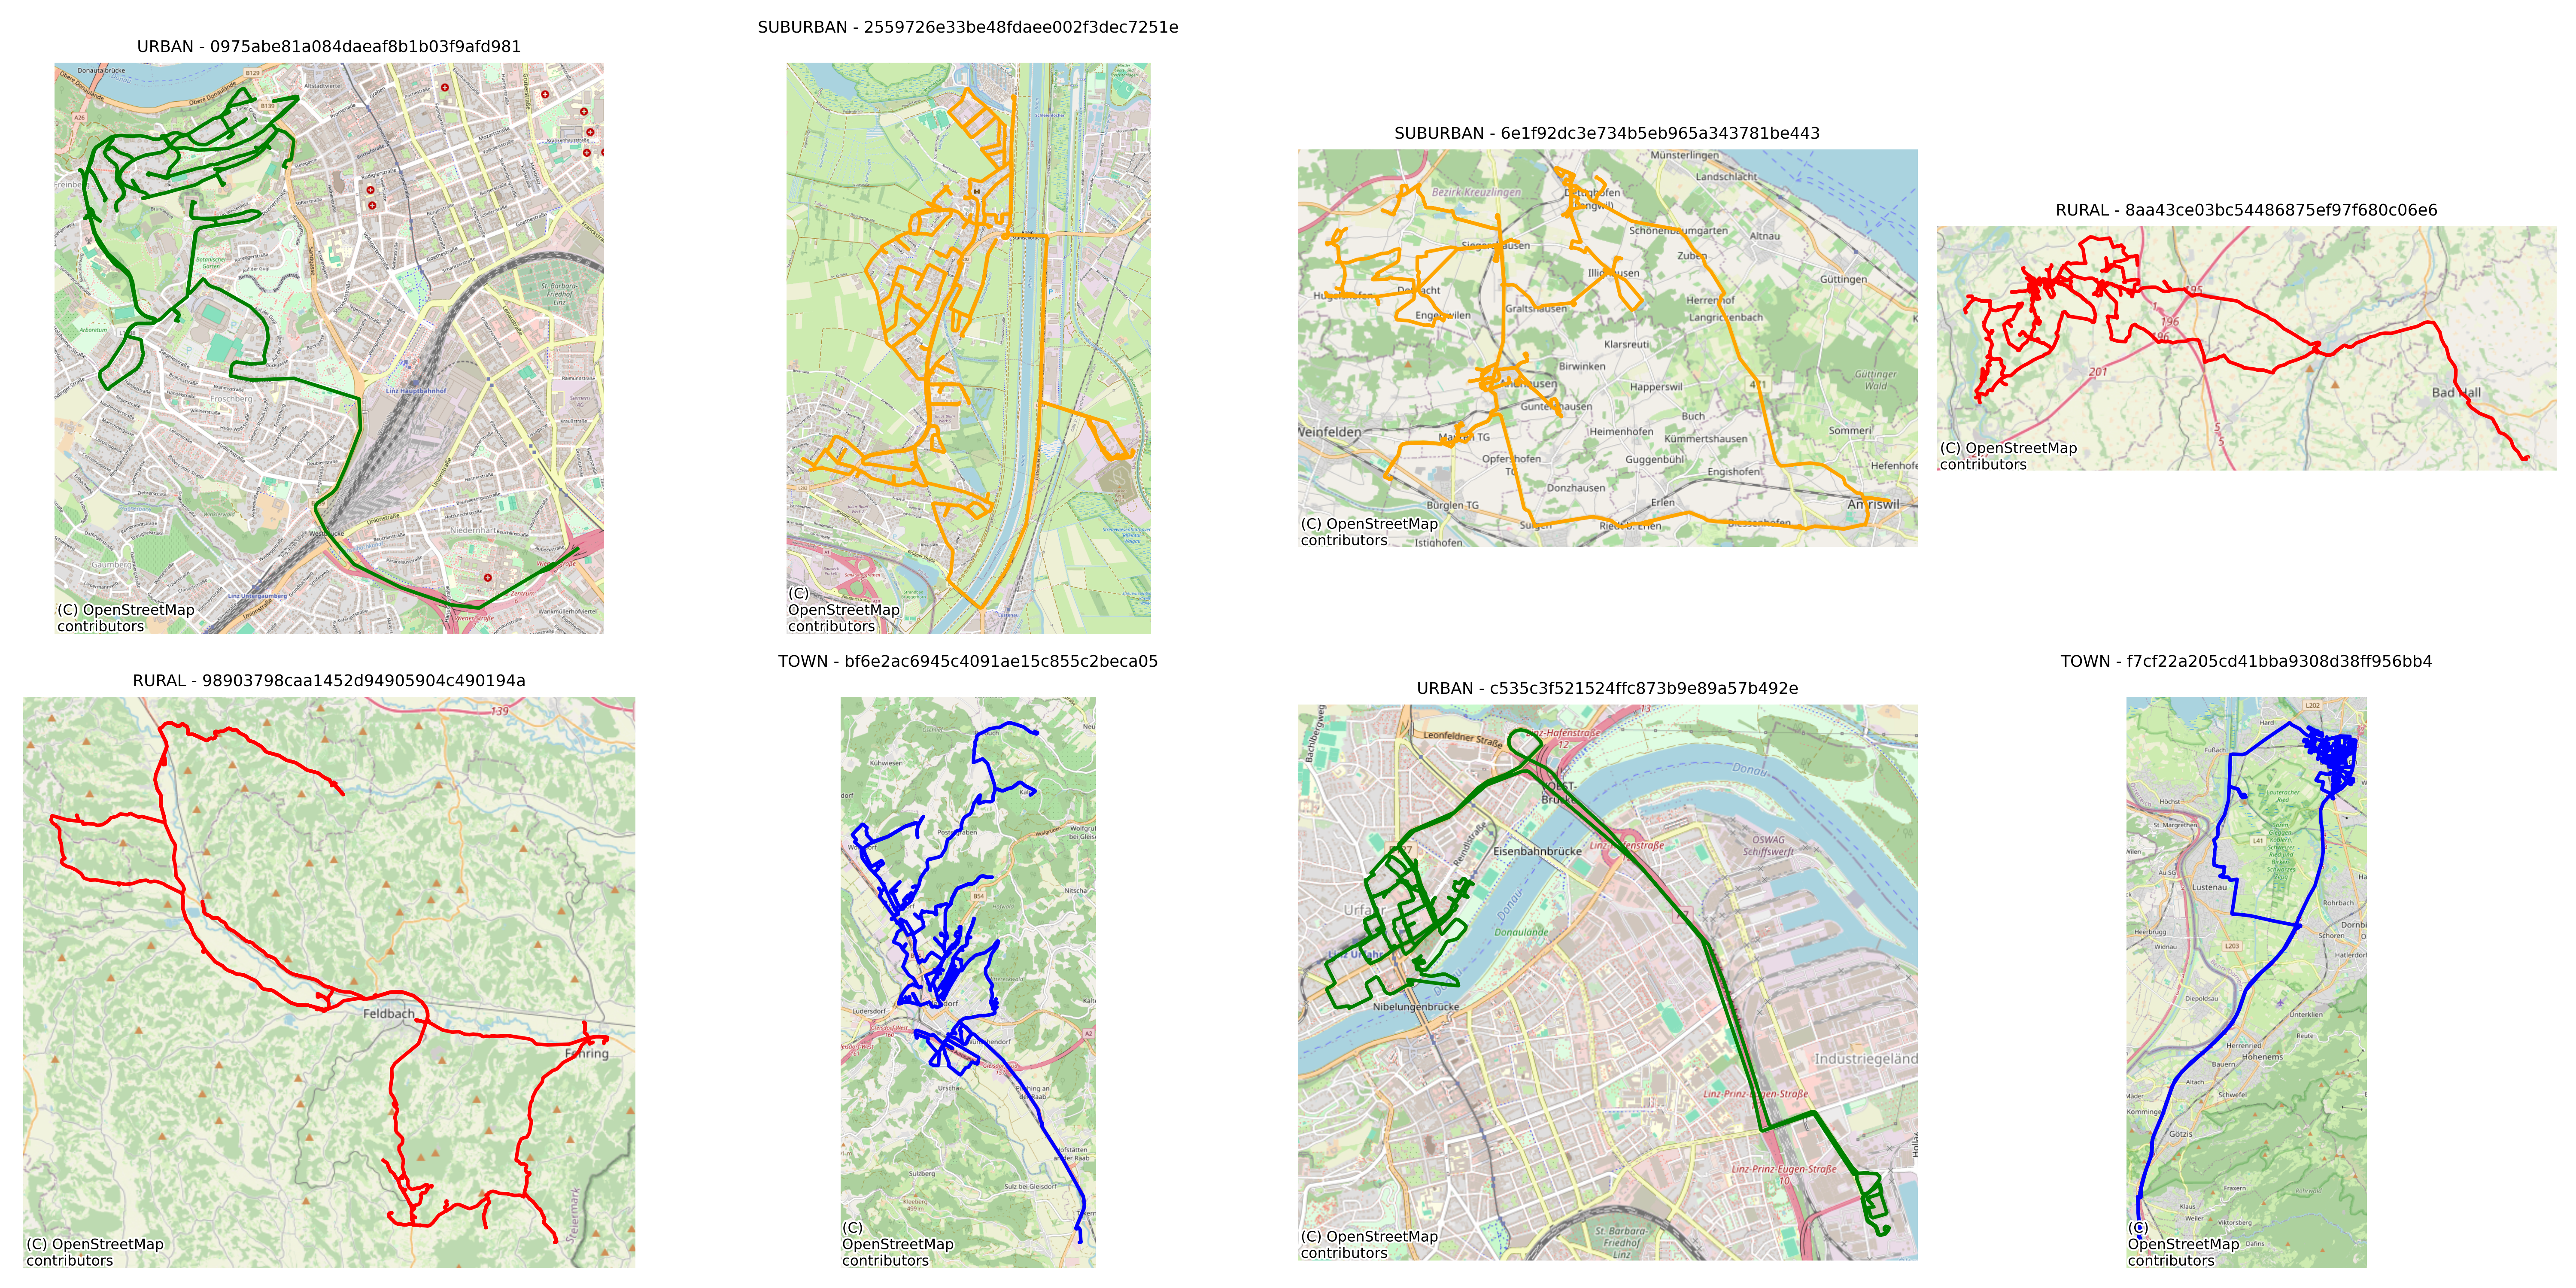
\includegraphics[width=\textwidth]{Figures/sample_tracking_routes_mapgrid.png}
  \caption{Mapgrid for selected sample trackings}
  \label{fig:sample_mapgrid}
\end{figure}
\FloatBarrier
The mapgrid shows spatial layout of each tracking route overlayed on a visual
map. Each subplot corresponds to a single tracking and is colorcoded with the
assigned lable (RURAL=Red, SUBURBAN=Orange, TOWN=Blue, URBAN=Green). This
visual representation clearly shows the difference in route shapes and sizes
between the four different area types.

\textbf{Urban:}
\begin{itemize}
  \item Routes are geographically compact and highly localized.
  \item Movement appears dense with short travel distances between stops.
  \item Often confined to a small cluster of city blocks or neighborhoods.
\end{itemize}

\textbf{Town:}
\begin{itemize}
  \item Coverage is slightly more dispersed than urban routes.
  \item Still relatively compact but less tightly packed.
  \item Serves a central area and nearby residential surroundings.
\end{itemize}

\textbf{Suburban:}
\begin{itemize}
  \item Routes extend farther and cover wider areas than town routes.
  \item Show transitional behavior between urban and rural structures.
  \item Less dense stop distribution, indicating more spaced-out residential
        zones.
\end{itemize}

\textbf{Rural:}
\begin{itemize}
  \item Routes are long and span large geographical areas.
  \item Stops are widely spaced, often connecting small, isolated settlements.
  \item The shape and path vary significantly, often following main roads
        between distant collection points.
\end{itemize}

\begin{figure}[htbp]
  \centering
  \includegraphics[width=\textwidth]{Figures/sample_pairplot.png}
  \caption{Pairplot of selected GPS route features grouped by area label}
  \label{fig:sample_pairplot}
\end{figure}
\FloatBarrier

The pairplot compares the relationships between the extracted features (eg.,
length, duration, number of points, bounding box area, point density, average
segmengt distance and number of stops). Rural and urban trackings show a clear
difference in multiple features. Point density and average segment distance are
especially good discriminators. Suburban and town trackings show more variance
and occasionally overlap with eachother, giving a not so clear distinction.

\begin{figure}[htbp]
  \centering
  \includegraphics[width=\textwidth]{Figures/sample_correlation_matrix.png}
  \caption{Correlation Matrix of selected GPS route features grouped by area
    label}
  \label{fig:sample_correlation_matrix}
\end{figure}
\FloatBarrier

The Correlation Matrix highlights the strong correlations between features in
the selected sample.
A high posive correlation between length, duration and number of points can be
observerd. Additionally the point density has a strong negative correlation
with the tracking length, number of points and average segment distance.

This correlation is to be expected and confirms the consistency of the data,
since the points (GPS coordinates) are recorded in uniform intervals. This plot
also indicates the possible redundance of features such as number of points and
number of stops.

\begin{figure}[h]
  \centering

  \includegraphics[width=\textwidth]{Figures/sample_point_density_boxplot.png}
  \caption{Boxplot of point density grouped by area label}
  \label{fig:sample_boxplot}
\end{figure}
\FloatBarrier

The point density boxplots for each label shows a clear difference between the
labels. Urban trackings appear to have the highest density and rural trackings
the lowest, with suburban and town trackings falling in the middle with a wider
variability.

This validates that the point density is a strong feature for classifying
trackings to the four labels.

\section{Solution Approach}
Formatvorlage für den Fließtext.

\chapter{Implementation}

\section{Implementation of the Big Picture}
Formatvorlage für den Fließtext.

\section{Integration with existing systems}
Formatvorlage für den Fließtext.

\chapter{Evaluation and Discussion}

\section{Definition of the data sets used for the evaluation}
Formatvorlage für den Fließtext.

\section{Evaluation of the results}
Formatvorlage für den Fließtext.

\section{Reflection on the results}
Formatvorlage für den Fließtext.

\chapter{Conclusion}

\section{Future Directions}
Formatvorlage für den Fließtext.

\section{Limitations}
Formatvorlage für den Fließtext.

% Literaturverzeichnis:
\clearpage
\phantomsection
\addcontentsline{toc}{chapter}{Literaturverzeichnis}
\printbibliography

\chapter*{[evtl. Anhang]}  % evtl. ersetzen mit \chapter*{Anhang}
\addcontentsline{toc}{chapter}{[evtl. Anhang]}
% evtl. ersetzen mit \addcontentsline{toc}{chapter}{Anhang}
Formatvorlage für den Fließtext.

\section{Use of AI tools}
\begin{table}[htbp]
  \centering
  \caption{Use of AI tools during the creation process}
  \label{tab:ai_usage}
  \begin{tabular}{|p{5.2cm}|c|c|p{6.2cm}|}
    \hline
    \textbf{Working step}                  & \textbf{AI used}       &
    \textbf{AI
    tool(s)}                               &
    \textbf{Experiences / recommendations / irritations}
    \\
    \hline
    Find a topic idea                      & no                     & -
                                           & -
    \\
    Narrow down topic / Formulate question & no                     & -
                                           & -
    \\
    Find sources                           & yes                    & Openai
    GPT-4o
                                           & Helped identify
    relevant keywords and topic clusters.
    \\
    Explain terms                          & yes                    & Openai
    GPT-4o
                                           & Useful for quick
    definitions and simple explanations.
    \\
    Design text structure                  & yes                    & Openai
    GPT-4o
                                           & Good for outlining
    sections. Required manual adjustments.
    \\
    Have content read aloud                & no                     & -
                                           & -
    \\
    Translate content                      & no                     & -
                                           & -
    \\
    Dictate content                        & no                     & -
                                           & -
    \\
    Paraphrase content, summarise          & yes                    & Openai
    GPT-4o
                                           & Helpful to generate
    concise summaries of long text.
    \\
    Write introduction                     & yes                    & Openai
    GPT-4o
                                           & Provided inspiration
    but required rewording.
    \\
    Write main chapter                     & yes                    & Openai
    GPT-4o
                                           & Used for structuring
    and rephrasing, not full writing.
    \\
    Write a summary                        & yes                    & Openai
    GPT-4o
                                           & Used to condense main
    points effectively.
    \\
    Obtain text feedback                   & yes                    & Openai
    GPT-4o
                                           & Used to review tone,
    clarity, and consistency.
    \\
    Revise text statement                  & yes                    & Openai
    GPT-4o
                                           & Helpful for
    reformulating statements.
    \\
    Revise text formulation                & yes                    & Openai
    GPT-4o
                                           & Polished sentences and
    improved flow.
    \\
    Correct text formally                  & yes                    & Openai
    GPT-4o
                                           & Assisted with grammar
    and punctuation checking.
    \\
    \hline
  \end{tabular}
\end{table}

\chapter*{Affidavit}
\addcontentsline{toc}{chapter}{Affidavit}
I hereby declare in lieu of oath that I have written this Bachelor
thesis independently and without the use of aids other than those specified.
The passages taken directly or indirectly from other sources
directly or indirectly from other sources are marked as such. The thesis has
not been
neither in the same nor in a similar form to any other examination authority
nor has it been published.

\vspace{3cm}
\noindent
Dornbirn, on 15. May 2025\hfill Matthias Hefel

\end{document}
